\chapter{Implementation}
In computer graphics, we generally synthesize 2d images from a given 3d scene description$\footnote{A usual computer graphics scene consist of a viewer's eye, modeled by a virtuel camera, light sources and geometries placed in the world, having some material properties assigned to.}$. This process is denoted as rendering. A usual computer graphics scene consist of a viewer's eye, modeled by a virtuel camera, light sources and geometries placed in the world$\footnote{With the term world we are refering to a global coordinate system which is used in order to place all objects.}$, having some material properties$\footnote{Example material properties are: textures, surface colors, reflectance coefficients, refractive indices and so on.}$ assigned to. In our implementation, scene geometries are modeled by triangular meshes for which each triangle is represented by a triple of vertices. Each vertex has a position, a surface normal and a tangent vector associated with. \\

The process of rendering basically involves a mapping of 3d sceene objects to a 2d image plane and the computation of each image pixel's color according to the provided lighting, viewing and material information of the given scene. These pixel colors are computed in several statges in so called shader programs, directly running on the Graphic Processing Unit (GPU) hardware device. In order to interact with a GPU, for our implementations, we rely on the programing interface of OpenGL$\footnote{Official website:\texttt{http://www.opengl.org/}}$, a cross-language, multiplattform API. In OpenGL, there are two fundamental shading pipeline stages, the vertex- and the fragment shading stage, each applied sequentially. Vertex shaders apply all transformations to the mesh vertices and pass this data to the fragment shaders. Fragment shaders receive linearly interpolated vertex data of a particular triangle. They are responsible to compute the color of his triangle. \\

In this chapter we explain in detail a technique for rendering structural colors due to diffraction effects on natural graings, based on the model we have derived in the previouse chapter $\ref{chap:derivations}$, summarized in section $\ref{sec:spectralrendering}$. For this purpose we implemented a reference framework which is based on a class project of the lecture \emph{Computer Graphics} held by Mr. M. Zwicker which I attended in autum 2012$\footnote{The code of underlying reference framework is written in Java and uses JOGL and GLSL$\footnotemark$ in order to comunicate with the GPU and can be found at \texttt{https://ilias.unibe.ch/}}$. \\
$\footnotetext{JOGL is a Java binding for OpenGL (official website \texttt{http://jogamp.org/jogl/www/}) and GLSL is OpenGL's high-level shading language. Further information can be found on wikipedia: \texttt{http://de.wikipedia.org/wiki/OpenGL\textunderscore Shading\textunderscore Language}}$

For performing the rendering process, our implementation expects being provided by the following input data$\footnote{All data is provided by the Laboratory of Artificial and Natural Evolition in Geneva. See their website:\texttt{www.lanevol.org}}$:
\begin{itemize}
  \item the structure of snake skin of different species$\footnote{We are using height field data for Elaphe and Xenopeltis snakes individuals like shown in figure $\ref{fig:snakespecies}$}$ represented as discrete valued height fields acquired using AFM and stored as grayscale images.
  \item real measured snake geometry represented as a triangle mesh.
\end{itemize}

The first processing stage of our implementation is to compute the Fourier Terms of the provided height fields like described in section $\ref{sec:taylorapproximation}$. For this preprocessing purpose we use Matlab relying on its internal, numerically fast, libraries for computing Fourier Transformations$\footnote{Actually we use Matlab's inverse 2d Fast Fourier Transformation (FFT) implementation applied on different powers of quation $\ref{eq:px}$. Further information can be read up in section $\ref{sec:precompmatlabfourierimages}$}$. The next stage is to read these precomputed Fourier Terms into our Java renderer. This program also builds our manually defined rendering scene. The last processing stage of our implementation is rendering of the iridescent colorpatterns due to light diffracted on snake skins. We implemented our diffraction model from chapter $\ref{chap:derivations}$ as OpenGL shaders. Notice that all the necessary computations in order to simulate the effect of diffraction are performed within a fragment shader. This implies that we are modeling pixelwise the effect of diffraction and hence the overall rendering quality and runtime complexity depends on rendering window's resolution. \\

In the following sections of this chapter we are going to explain all render processing stages in detail. First, we discuss, how our precomputation process, using Matlab, actually works. Then, we introduce our Java Framework. It is followed by the main section of this chapter, the explanation how our OpenGL shaders are implemented. The last section discusses an optimization of our fragment shader such that it will have interactive runtime.

\section{Precomputations in Matlab}
\label{sec:precompmatlabfourierimages}
Our first task is to precompute the two dimensional discrete Fourier Fransformations$\ref{eq:dftnterm}$ for a given height field, representing a natural grating. For that purpose we have written a small Matlab $\footnote{Matlab is a interpreted scripting language which offers a huge collection of mathematical and numerically fast and stable algorithms.}$ script conceptialized algorithmically in $\ref{alg:matlabprecomp}$. Our Matlab script reads a given image, which is representing a nano-scaled height field, and computes its two dimensional DFT (2dDFT) by using Matlab's internal Fast Fourier Transformation (FFT) function, denoted by $ifft2$$\footnote{Remember, even we are talking about fourier transformations, in our actual computation, we have to compute the inverse fourier transformation. See paragraph $\ref{sec:electricalengeneeringftconvention}$ for further information. Furthermore our height fields are two dimensional and thus we have to compute a 2d inverse fourier transformation.}$. Note that we only require one color channel of the input image, since the input image is representing an height field, encoded by just one color. Keep in mind that taking the Fourier transformation of an arbitrary function will result in a complex valued output which implies that we will get a complex value for frequency pairs of our input image. Therefore, for each input image we get as many output images, representing the 2dDFT, as the minimal number of taylor terms required for a well-enough approximation. In order to store our output images, we have to use two color channels instead of just one like it was for the given input image. Some example visualizations for the Fourier Tranformation are shown in figure $\ref{fig:matlabBlazeFourierImages}$. We store these intermediate results as binary files to offer floating point precision for the run-time computations to ensure higher precision. \\

In our script every discrete frequency is normalized by its corresponding DFT extrema$\footnote{We are talking about the i2dFFT of our height fields to the power of n. This is an N by N matrix (assuming the discrete height field was an N by N image), for which each component is a complex number. Hence, there is a a complex extrema as well as a imaginary extrema.}$ in the range $\left[0,1\right]$ and the range extrema are stored seperately for each DFT term. The normalization is computed the following way: 

\begin{align}
  f:\left[x_{min},x_{max}\right]\to \left[0,1\right] \nonumber\\
  x \mapsto f(x) = \frac{x-x_{min}}{x_{max}-x_{min}}
\label{eq:dfttermnormalization}
\end{align}
Where $x_{min}$ and $x_{max}$ denote the extreme values of a DFT term. Later, during the shading process of our implementation, we have to apply the inverse mapping. This is non-linear interpolation which is required in order to rescaled all frequency values in the DFT terms. 

\begin{algorithm}[H]
\caption{Precomputation: Pseudo code to generate Fourier terms}
\textbf{INPUT} \ $heightfieldImg, \ maxH, \ dH, \ termCnt$ \\
\textbf{OUTPUT} \ $DFT \ terms \ stored \ in \ Files$
\begin{lstlisting}
% maxH:    A floating-point number specifying 
%          the value of maximum height of the 
%          height-field in MICRONS, where the 
%          minimum-height is zero. 
%         
% dH:      A floating-point number specifying 
%          the resolution (pixel-size) of the 
%          'discrete' height-field in MICRONS. 
%          It must be less than 0.1 MICRONS 
%          to ensure proper response for 
%          visible-range of light spectrum.
%
% termCnt: An integer specifying the number of 
%          Taylor series terms to use.

function ComputeFFTImages(heightfieldImg, maxH, dh, termCnt)
dH = dh*1E-6;
% load patch into heightfieldImg
patchImg = heightfieldImg.*maxH;
% rotate patchImg by 90 degrees
for t = 0 : termCnt
  patchFFT = power(1j*patchImg, t);
  fftTerm{t+1} = fftshift(ifft2(patchFFT));
  
  % rescale terms as
  imOut(:,:,1)  = real(fftTerm{t+1});
  imOut(:,:,2)  = imag(fftTerm{t+1});
  imOut(:,:,3)  = 0.5;
  
  % rotate imOut by -90 degrees
  % find real and imaginary extrema of 
  % write imOut, extrema, dH, into files.
end
\end{lstlisting}
\label{alg:matlabprecomp}
\end{algorithm}

The command fftshift rearranges the output of the ifft2 by moving the zero frequency component to the centre of the image. This simplifies the computation of DFT terms lookup coordinates during rendering.

\label{sec:precompmatlabfft}
\begin{figure}[H]
  \centering
  \subfigure[Blaze Patch]{
    
\includegraphics[scale=0.25]{implementation/hf/blaze/blazeBig.png}
    \label{fig:matlabBlazePatch}
  }
~
  \subfigure[Extrema Plot]{
    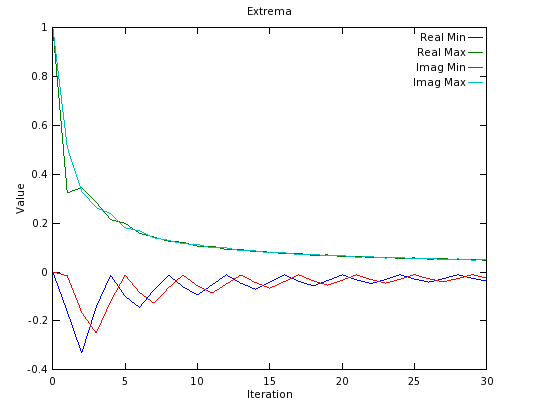
\includegraphics[scale=0.4]{implementation/hf/blaze/extrema.png}
    \label{fig:extremaBlaze}  
  }
  
  \subfigure[ImRe0]{
    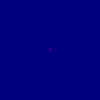
\includegraphics[scale=0.6]{implementation/hf/blaze/AmpReIm0.png}
    \label{fig:blazeftimre0}
  }
~
  \subfigure[ImRe1]{
    
\includegraphics[scale=0.6]{implementation/hf/blaze/AmpReIm1.png}
    \label{fig:blazeftimre1}
  }
~
  \subfigure[ImRe4]{
    
\includegraphics[scale=0.6]{implementation/hf/blaze/AmpReIm4.png}
    \label{fig:blazeftimre4}
  }
~
  \subfigure[ImRe10]{
    
\includegraphics[scale=0.6]{implementation/hf/blaze/AmpReIm10.png}
    \label{fig:blazeftimre10}
  }
~
  \subfigure[ImRe20]{
    
\includegraphics[scale=0.6]{implementation/hf/blaze/AmpReIm20.png}
    \label{fig:blazeftimre20}
  }
 
  
  \subfigure[Re0]{
    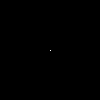
\includegraphics[scale=0.6]{implementation/hf/blaze/re0.png}
    \label{fig:blazeftre0}
  }
~
  \subfigure[Re1]{
    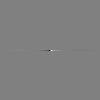
\includegraphics[scale=0.6]{implementation/hf/blaze/re1.png}
    \label{fig:blazeftre1}
  }
~
  \subfigure[Re4]{
    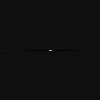
\includegraphics[scale=0.6]{implementation/hf/blaze/re4.png}
    \label{fig:blazeftre4}
  }
~
  \subfigure[Re10]{
    
\includegraphics[scale=0.6]{implementation/hf/blaze/re10.png}
    \label{fig:blazeftre10}
  }
~
  \subfigure[Re20]{
    
\includegraphics[scale=0.6]{implementation/hf/blaze/re20.png}
    \label{fig:blazeftre20}
  }
  
  \subfigure[Im0]{
    
\includegraphics[scale=0.45]{implementation/hf/blaze/im0.png}
    \label{fig:blazeftim0}
  }
~
  \subfigure[Im1]{
    
\includegraphics[scale=0.6]{implementation/hf/blaze/im1.png}
    \label{fig:blazeftim1}
  }
~
  \subfigure[Im4]{
    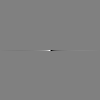
\includegraphics[scale=0.6]{implementation/hf/blaze/im4.png}
    \label{fig:blazeftim4}
  }
~
  \subfigure[Im10]{
    
\includegraphics[scale=0.6]{implementation/hf/blaze/im10.png}
    \label{fig:blazeftim10}
  }
~
  \subfigure[Im20]{
    
\includegraphics[scale=0.6]{implementation/hf/blaze/im20.png}
    \label{fig:blazeftim20}
  }
  
  \caption{Blaze}
  \label{fig:matlabBlazeFourierImages}
\end{figure}

In figure $\ref{fig:matlabBlazeFourierImages}$ we see some Fourier images rendered by our Matlab script for the blaze grating $\ref{fig:matlabBlazePatch}$ used as input image. For example figure $\ref{fig:blazeftimre4}$ represents the two dimensional Fourier transform of the input image to the power of four times the imgaginary number $i$ stored in a RGB image. Note that the red color channel $\ref{fig:blazeftre4}$ contains the real- and the green color channel $\ref{fig:blazeftre4}$ the imaginary part of the Fourier transform. The plot in figure $\ref{fig:extremaBlaze}$ shows the development of blaze grating's extreme values for different powers. 

\section{Java Renderer}
In autumn 2012, during the semester I have attented the class computer graphics held by M. Zwicker where we have developed a real time renderer program written in java. The architecture of the program is divided into two parts: a rendering engine, the so called jrtr (java real time renderer) and an application program. Figure $\ref{fig:rendererArchitecture}$ outlines the architecture of our renderer. 

\begin{figure}[H]
  \centering
  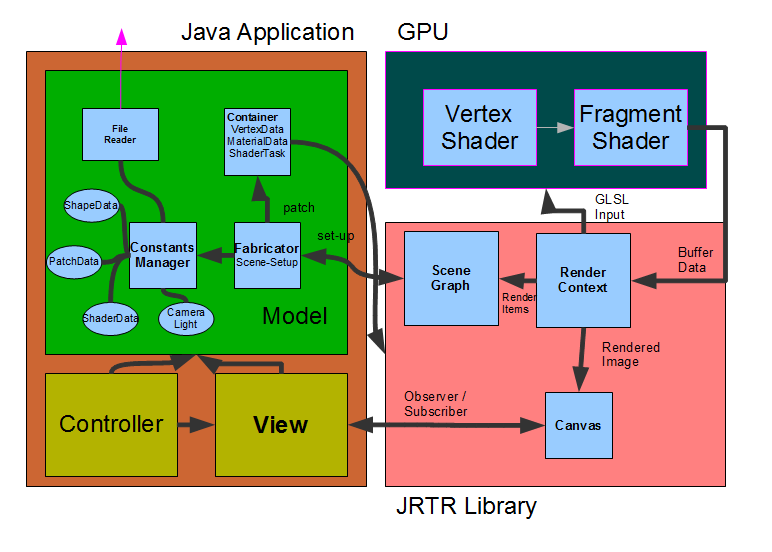
\includegraphics[scale=0.7]{implementation/framework.png}
  \caption{Renderer Architecture}
  \label{fig:rendererArchitecture}
\end{figure}

The application program relies on the MVC (Model-View-Controller) architecture pattern. The View just represents a canvas in which the rendered images are shown. The Controller implements the event listener functionalities in order manipulate the rendered shape within the canvas. The Model of our application program consists of a Fabricator, a file reader and a constants manager. The main purpose of a Fabricator is to set up a rendering scene by accessing a constant manager containing many predefined scene constants. A scene consists of a camera, a light source, a frustum, shapes and their associated material constants. Such materials contain a shape's texture, associated Fourier images $ref{fig:matlabBlazeFourierImages}$ for a given height field and other height field constants such as the maximal height of a bump. A shapes is a geometrical object defined by a wireframe mesh as shown in figure $\ref{fig:wireframemesh}$. 

\begin{figure}[H]
  \centering
  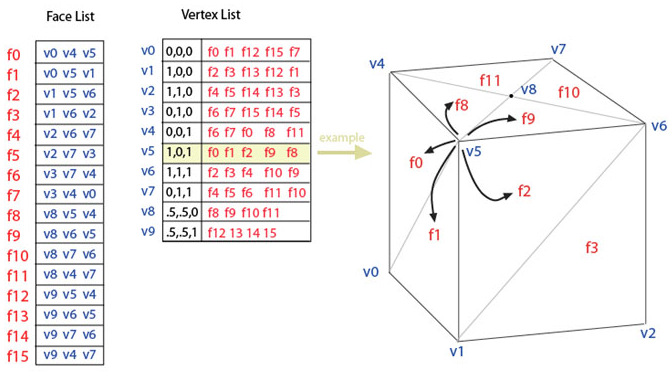
\includegraphics[scale=0.7]{implementation/wireframemesh.png}
  \caption{A wireframe mesh represents an object as a set of faces and a set of vertices.}
  \label{fig:wireframemesh}
\end{figure}

Such a mesh is a special data structure consisting of vertices, each stored as a triple of $xyz$ positions in an float array and triangles, each defined by a triple of vertex-indices which form a fragment each stored in an integer array. It is also possible to assign additional geometry data like a color, normals and texture coordinates associated to each vertex. \\

The whole scene is stored within container data-structures, defined and managed within jrtr. In our case we rely on a scene graph, which contains all geometries and their transformations in a tree like structured hierarchy. The geometries are stored within an container, including all vertex attributes and the material constants. The jrtr rendering engine uses a low-level API, called OpenGL in order to communicate with the graphics processor unit (GPU) where the actual shading happens. Within jrtr's render context object, the whole resource-management for the rendering pipeline takes place. This means all required low-level buffers are allocated, flushed and assigned by the scene data attributes. The GPU's rendering pipeline will use those buffers for its shading process. Its first stage is the vertex shader $\ref{sec:vertexshader}$ followed by the fragment shader $\ref{sec:fragmentshader}$. The jrtr framework also offers the possibility to assign arbitrary shaders.

\section{GLSL Diffraction Shader}
\subsection{Vertex Shader}
\label{sec:vertexshader}
The Vertex shader is the first shading stage within our rendering pipeline and responsible for computing all necessary per vertex data. Usually, within a vertex shader each vertex position is transformed into a projective space:

\begin{equation}
  p_{projective} = P \cdot C^{-1} \cdot M \cdot p_{obj}
\end{equation}

Where M is a transformation from the local object space to the reference coordinate system, called world space, $C^{-1}$ camera matrix C and $P$ the projection matrix. The camera matrix defines transformation from camera to world coordinates as shown in figure $\ref{fig:cameracoordinatesystem}$.

\begin{figure}[H]
  \centering
  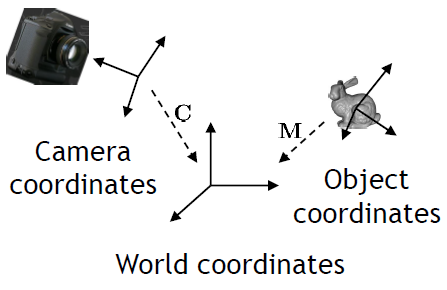
\includegraphics[scale=0.7]{implementation/cameracoodsyst.png}
  \caption{Camera coordinate system where its origin defines the center of projection of camera}
  \label{fig:cameracoordinatesystem}
\end{figure}

The camera matrix is constructed from its center of projection $e$, the position the cameras looks at $d$ and up vector denoted by $up$ given in world coordinates like illustrated in figure $\ref{fig:cameramatrix}$

\begin{figure}[H]
  \centering
  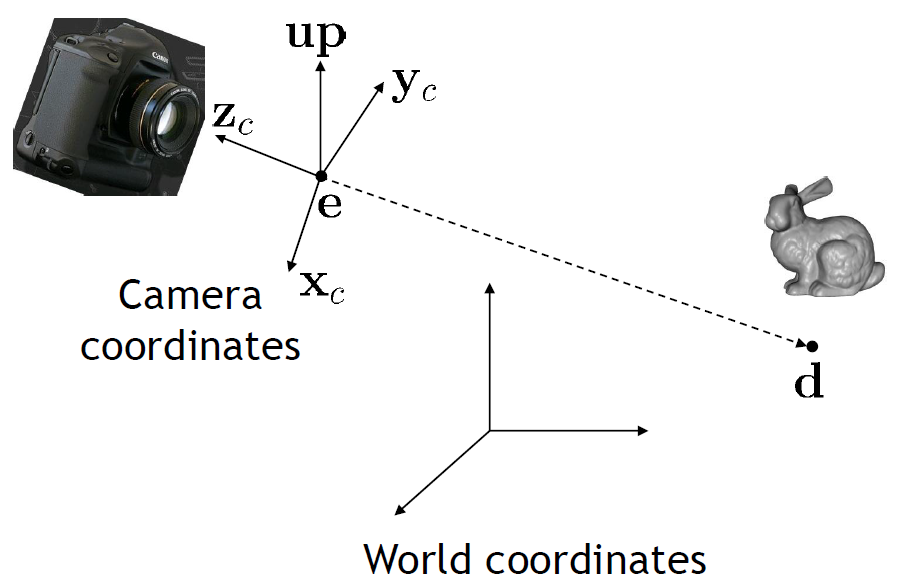
\includegraphics[scale=0.35]{implementation/cameramatrix.png}
  \caption{Illustration of involved components in order to construct the camera matrix. We introduce some helper vectors $z_c = \frac{e-d}{||e-d||}$, $x_c = \frac{up \times z_c}{||up \times z_c||} $ and $z_c \times x_c$ for the actual construction of the camera matrix}
  \label{fig:cameramatrix}
\end{figure}

The mathematical representation of the camera matrix, using the helper vectors introduced in figure $\ref{fig:cameramatrix}$, looks like:

\begin{equation}
C = \begin{bmatrix} x_c & y_c & z_c & e \\ 0 & 0 & 0 & 1 \end{bmatrix}
\end{equation}

All vertex shader output will be used within the fragment shader $\ref{sec:fragmentshader}$. In our vertex shader we also compute for every vertex in our current geometry the direction vectors $\omega_i$ and $\omega_r$ described like in figure $\ref{fig:geometricsetup}$. Those direction vectors are transformed onto the tangent space, a local coordinate system spanned by a vertex's normal, tangent and binormal vector. Have a look at the appendix $\ref{sec:tangentspace}$ for further information and insight about the tangent space. The algorithm $\ref{alg:vertexshader}$ stated below shows our vertex shader.
  
\begin{algorithm}[H]
  \caption{Vertex diffraction shader pseudo code}
  \begin{algorithmic}
    \INPUT $N, T, Shape, lightDir$
    \MOUTPUT $Structural Color on Fragment$
    \ForAll{$Vertex \thinspace v \in Shape$}
      \State $ vec3 \ N = normalize(modelM * vec4(normal,0.0).xyz)$
      \State $ vec3 \ T = normalize(modelM * vec4(tangent,0.0).xyz)$
      \State $ vec3 \ B = normalize(cross(N, T))$
      \State $ vec3 \ Pos = ((cop_{w}-position)).xyz$
      \State $ lightDir = normalize(lightDir)$
      \State $ l = projectVectorOnTo(lightDir, TangentSpace)$
      \State $ p = projectVectorOnTo(Pos, TangentSpace)$
      \State $normalize(l); normalize(p)$
      \State $p_{per} = P \cdot C^{-1} \cdot M \cdot p_{obj}$
    \EndFor
  \end{algorithmic}
\label{alg:vertexshader}
\end{algorithm}

As already mentioned in section $\ref{sec:dirlighsourceassumption}$, our light source is a directional light source (See figure $\ref{fig:dirlightsource}$).

\begin{figure}[H]
  \centering
  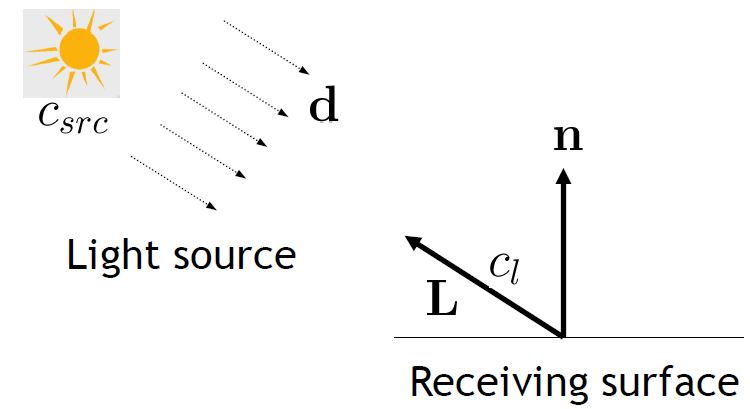
\includegraphics[scale=0.45]{implementation/dirlightsource.png}
  \caption{For a directional light source all light rays are in parallel.}
  \label{fig:dirlightsource}
\end{figure}

\subsection{Fragment Shader}
\label{sec:fragmentshader}
The purpose of a fragment shader is to render per fragment. A fragment is spanned by three vertices of a given mesh. For each pixel within a fragment in the fragment shader, the output of from its spanning vertices computed in the vertex shaders $\ref{alg:vertexshader}$ is trilinearly interpolated depending on the pixel's position within the fragment. Furthermore, there can be additional input be assigned which is not directly interpolated from the output of vertex shader programs. In our fragment shader $\ref{alg:fragmentshaderall}$ this will be: all the references to the image buffers, containing the Fourier images computed in Matlab $\ref{sec:precompmatlabfourierimages}$, the number steps for the taylor approximation (in our shader 30), the minimal and maximal wavelength, scaling factors, a reference to a lookup table containing the $CIE_{XYZ}$ color weights. Basically the whole computation within our fragment shader relies on the direction of light and the viewing direction. Our shader performs a numerical integration for our final derived expression in equation $\ref{eq:finalexpression}$ using the trapezoidal-rule with uniform discretization of the wavelength spectrum at $5nm$ step sizes. This implies we are compressing sampled frequencies to the region near to the origin of their frequency domain due to the fact we are dividing the $(u,v)$ by the wavelength and this implies that the $(u,v)$ space is sampeled non-linearly. \\

The Gaussian window approach derived in section $\ref{sec:gaussianwindow}$ is performed for each discrete $\lambda$ value using a window large enough to span $4\sigma_f$ in both dimensions. For precomputing DFT tables we generally use nanostructure height fields that span at least 65$\mu m^2$ and are sampled with resolution of at least 100nm. This ensures that the spectral response encompasses all the wavelengths in the visible spectrum, i.e. from 380nm to 780nm.

\begin{algorithm}[H]
  \caption{Fragment diffraction shader pseudo code}
  \begin{algorithmic}[1]
    \INPUT $Precomputed \thinspace DFT \thinspace Terms,\thinspace Scene \thinspace Geometry$
    \MOUTPUT $Structural Color on Fragment$
    \ForAll{$Pixel \thinspace p \in Fragment$}
      \State \init $BRDF_{XYZ}, BRDF_{RGB}$ \myto $vec4(0.0)$
      \State $(u,v,w) = -\omega_i - \omega_r$
      \For{$(\lambda = \lambda_{min};\thinspace \lambda \leq \lambda_{max};\thinspace \lambda = \lambda + \lambda_{step})$}
        \State $xyzWeights = ColorWeights(\lambda)$
        \State $lookupCoord = lookupCoord(u, v, \lambda)$
        \State \init $P$ \myto $vec2(0.0)$
        \State $k = \frac{2\pi}{\lambda}$
        \For{$(n = 0$ \myto $T)$}
          \State $taylorScaleF = \frac{(kw)^n}{n!}$
          \State \init $F_{fft}$  \myto $vec2(0.0)$
          \State $anchorX = int(floor(center.x + lookupCoord.x * fftImWidth)$
          \State $anchorY = int(floor(center.y + lookupCoord.y * fftImHeight)$
          \For{$(i=(anchorX-winW)$ \myto $(anchorX + winW))$}
            \For{$(j=(anchorY - winW)$ \myto $(anchorY + winW))$}
              \State $dist = distVecFromOriginTo(i,j)$
              \State $pos = localLookUp(i,j,n)$
              \State $fftVal = rescaledFourierValueAt(pos)$
              \State $fftVal \asteq gaussWeightOf(dist)$
              \State $F_{fft} \pluseq fftVal$
            \EndFor
          \EndFor
          \State $P \pluseq taylorScaleF*F_{fft}$
        \EndFor
        \State $xyzPixelColor \pluseq dot(vec3(\left|P\right|^2), xyzWeights)$
      \EndFor
      \State $BRDF_{XYZ} = xyzPixelColor*C(\omega_i, \omega_r)*shadowF$
      \State $BRDF_{RGB}.xyz = D_{65}*M_{XYZ-RGB}*BRDF_{XYZ}.xyz$
      \State $BRDF_{RGB}= gammaCorrect(BRDF_{RGB})$
    \EndFor
  \end{algorithmic}
  \label{alg:fragmentshaderall}
\end{algorithm}


\myparagraph{From line 4 to 26:} 
This loop performs uniform sampling along wavelength-space. $ColorWeights(\lambda)$ computes the color weight for the current wavelength $\lambda$ by linear interpolation between the color weight for $\ceil{\lambda}$ and $\floor{\lambda}$ which are stored in a external weights-table (assuming this table contains wavelengths in 1nm steps). At line 6: $lookupCoord(u, v, \lambda)$ the coordinates for the texture lookup are computed - See $\ref{eq:scalelook}$. Line 25 sums up the diffraction color contribution for the current wavelength in iteration $\lambda$.  

\myparagraph{From line 9 to 24:} 
This loop performs the Taylor series approximation using T terms. Basically, the spectral response is approximated for our current $(u,v,\lambda)$. Furthermore, neighborhood boundaries for the gaussian-window sampling are computed, denoted as anchorX and anchorY.

\myparagraph{From line 14 to 22:} 
In this inner most loop, the convolution of the gaussian window with the DFT of the patch is performed. $gaussWeightOf(dist)$ computes the weights in equation $~\eqref{eq:gaussweight}$ from the distance between the current pixel's coordinates and the current neighbor's position in texture space. Local lookup coordinates for the current fourier coefficient $fftVal$ value are computed at line 17 and computed like described in $\ref{eq:gaussianwindowlook}$. The actual texture lookup is performed at line 18 using those local coordinates. Inside $rescaledFourierValueAt$ the values $fftVal$ is rescaled by its extrema, i,e. $(fftVal*Max + Min)$ is computed, since $fftVal$ is normalized $\ref{sec:precompmatlabfft}$. The current $fftVal$ values in iteration is scaled by the current gaussian weight and then summed to the final neighborhood FFT contribution at line 20.

\myparagraph{After line 26:} 
At line 27 the gain factor $C(\omega_i, \omega_r)$  $\ref{eq:cfact}$ is multiplied by the current computed pixel color like formulated in $\ref{eq:cpterm}$. The gain factor contains the geometric term $ref{eq:geometricterm}$ and the Fresnel term $F$. W approximate $F$ by the Schlick approximation $\ref{eq:schlickapprox}$, using an reactive index at 1.5 since this is close to the measured value from snake sheds.
Our BRDF values are scaled by s shadowing function as described in (SEE REFERENCES - PAPER), since most of the grooves in the snake skin nano-structures would from a V-cavity along the plane for a wave front with their top-edges at almost the same height.

Last, we transform our colors from the $CIE_XYZ$ colorspace to the $CIE_RGB$ space using the CIE Standard Illuminant D65, followed by a gamma correction. See $\ref{subsec:colortransformations}$ for further insight.

\section{Technical details}
\subsection{Texture lookup}
In a GLSL shader the texture coordinates are normalized which means that the size of the texture maps to the coordinates on the range $[0,1]$ in each dimension. By convention the the bottom left corner of an image has the coordinates $(0,0)$, whereas the top right corner has the value $(1,1)$ assigned. 

Given a nano-scaled surface patch P with a resolution $A$ by $A$ microns stored as an $N$ by $N$ pixel image $I$.
Then one pixel in any direction corresponds to $dH = \frac{A}{N} \mu m$. 
In Matlab we compute a series of $n$ output images $\{I_{out_1},...,I_{out_n}\}$ from $I$, which we will use for the lookup in our shader - See figure $\ref{fig:lookupexample}$. For the lookup we use scaled and shifted $(u,v)$ coordinates from $\ref{eq:uvw}$. 

Since the zero frequency component of output images was shifted towards the centre of each image, we have to shift $u$, $v$ to the center of the current $N$ by $N$ pixel image by a bias $b$. Mathematically, the bias is a constant value is computed the following:

\begin{align}
    b
    &= (N \% 2 == 0) \quad ? \quad \frac{N}{2} : \frac{N-1}{2}
\label{eq:bias}
\end{align}

\begin{figure}[H]
  \centering
  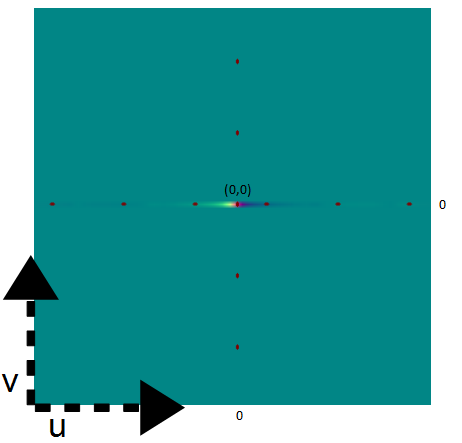
\includegraphics[scale=0.7]{implementation/lookupexampleAmReIm4.png}
  \caption{$(u,v)$ lookup image}
\label{fig:lookupexample}
\end{figure}

For the scaling we have to think a little further: lets consider a $T$ periodic signal in time, i.e. $x(t) = x(t+nT)$ for any integer n. After applying the DFT, we have its discrete spectrum $X[n]$ with frequency interval $w0 = 2pi / T$ and time interval $t0$. Let $k = \frac{2 \pi}{\lambda}$ denote the wavenumber for the current wavelength $\lambda$.
Then the signal is both periodic with time period $T$ and discrete with time interval $t_0$ then its spectrum should be both discrete with frequency interval $w_0$ and periodic with frequency period $\Omega = \frac{2 \pi}{t_0}$. This gives us the idea how to discretize the spectrum: Let us consider our Patch $P$ assuming it is distributed as a periodic function on our surface. Then, its frequency interval along the x direction is $w_0 = \frac{2 \pi}{T} = \frac{2 \pi}{N*dH}$. 
Thus only wave numbers that are integer multiples of $w_0$ after a multiplication with $u$ must be considered, i.e. $ku$ is integer multiple of $w_0$. Hence the lookup for the u-direction will look like:

\begin{align}
    \frac{ku}{w_0} 
    &= \frac{ku N dH}{2 \pi} \\
    &= \frac{u N dH}{\lambda}
\label{eq:scalelook}
\end{align}

Using those findings $\ref{eq:bias}$, $\ref{eq:scalelook}$, the final $(u,v)$ texture lookup-coorinates for the current wavelength $\lambda$ in iteration, will then look like:

\begin{equation}
  (u_{lookup}, v_{lookup}) = \left( \frac{u N dH}{\lambda} + b, \frac{v N dH}{\lambda} + b \right)
\label{eq:ublookup}
\end{equation}  

Note for the windowing approach we are visiting a one pixel neighborhood for each pixel $p$. 
This is like a base change with $(u_{lookup}, v_{lookup})$ as new coordinate system origin. The lookup coordinates for the neighbor-pixel $(i,j)$ are:

\begin{equation}
  (u_{lookup}, v_{lookup}) = (i,j)-(u_{lookup}, v_{lookup})
\label{eq:gaussianwindowlook}
\end{equation}

\subsection{Texture Blending}
The final rendered color for each pixel is a weighted average of different color components, such as the diffraction color, the texture color and the diffuse color. In our shader the diffraction color is weighted by a constant $w_{diffuse}$. the texture color is once scales by a binary weight determined by the absolute value of the Fresnel Term $F$ and once by $1-w_{diffuse}$. 

\begin{algorithm}[H]
  \caption{Texture Blending}
  \begin{algorithmic}
    \State $\alpha = (abs(F) > 1) ? 1 : 0$
    \State $c_{out} =(1-w_{diffuse})*c_{diffraction} + (1-\alpha)*c_{texture} + w_{diffuse}*c_{texture})$
  \end{algorithmic}
\end{algorithm}

\subsection{Color Transformation}
\label{subsec:colortransformations}

In our shader we access a table which contains precomputed CIE's color matching functions values from $\lambda_{min} = 380 nm$ to $\lambda_{max} = 780 nm$ in $5 nm$ steps. Such a function value table can be found at downloaded at cvrl.ioo.ucl.ac.uk for example. We compute the $(X,Y,Z)$ $CIE_{XYZ}$ color values as described in section $\ref{sec:colorspace}$. 


We can transform the color values into $CIE_{RGB}$ by performing the following linear transformation:

\begin{equation}
\begin{bmatrix}R\\G\\B\end{bmatrix} = M \cdot \begin{bmatrix}X\\Y\\Z\end{bmatrix}
\end{equation} 

where one possible transformation is: 

\begin{equation}
M = \begin{bmatrix} 0.41847 & -0.15866 & -0.082835\\ -0.091169 & 0.25243 & 0.015708\\ 0.00092090 & -0.0025498 & 0.17860 \end{bmatrix}
\end{equation}

There are some other color space transformation. The shader uses the CIE Standard Illuminant D65 which is intended to represent average daylight. Using D65 the whole colorspace transformation will look like:

\begin{equation}
\begin{bmatrix}R\\G\\B\end{bmatrix} = M \cdot \begin{bmatrix}X \cdot D65.x \\ Y \cdot D65.y \\Z \cdot D65.z \end{bmatrix} 
\end{equation}

Last we perfrom gamma correction on each pixel's $(R,G,B)$ value. Gamma correction is a non linear transformation which controls the overall brightness of an image.

\section{Discussion}
\label{sec:impldiscus}
The fragment shader algorithm described in $\ref{alg:fragmentshaderall}$ performs the gaussian window approach by sampling over the whole wavelength spectrum in uniform step sizes. This algorithm is valid but also slow since we iterate for each pixel over the whole lambda spectrum. Furthermore, for any pixel, we iterate over its 1 neighborhood. Considering the loop for the taylor approximation as well, we will have a run-time complexity of $O(\#spectrtumIter \cdot \#taylorIter \cdot neighborhoodRadius^2)$. 
Hence, Instead sampling over the whole wavelength spectrum, we could instead integrate over just a few required lambdas which are elicited like the following: Lets consider $(u,v,w)$ defined as $\ref{eq:uvw}$. Let $d$ be the spacing between two slits of a grating. For any $L(\lambda) \neq 0$ it follows $\lambda_{n}^{u} = \frac{d u}{n}$ and $\lambda_{n}^{v} = \frac{d u}{n}$. For $n = 0$ there it follows $(u,v)=(0,0)$. 
If $u,v > 0$
\begin{align*}
    N_{min}^{u} = \frac{d u}{\lambda_{max}} \leq n_{u} \leq \frac{d u}{\lambda_{min}} = N_{min}^{u}\\
    N_{min}^{v} = \frac{d v}{\lambda_{max}} \leq n_{v} \leq \frac{d v}{\lambda_{min}} = N_{min}^{v}
\end{align*}
If $u,v < 0$
\begin{align*}
    N_{min}^{u} = \frac{d u}{\lambda_{min}} \leq n_{u} \leq \frac{d u}{\lambda_{min}} = N_{max}^{u}\\
    N_{min}^{v} = \frac{d v}{\lambda_{min}} \leq n_{v} \leq \frac{d v}{\lambda_{min}} = N_{max}^{v}
\end{align*}

By transforming those equation to $(\lambda_{min}^{u}, \lambda_{min}^{u})$, $(\lambda_{min}^{v}, \lambda_{min}^{v})$ respectively for any $(u,v,w)$ for each pixel we can reduce the total number of required iterations in our shader.  

Another variant is the $PQ$ approach described in chapter 2 $\ref{sec:pq}$. Depending on the interpolation method, there are two possible variants we can think of as described in $\ref{sec:sincinterpolation}$. Either we try to interpolate linearly or use sinc interpolation.
The first variant does not require to iterate over a pixel's neighborhood, it is also faster than the gaussian window approach. One could think of a combination of those tho optimization approaches. Keep in mind, both of these approaches are further approximation. The quality of the rendered images will suffer using those two approaches. The second variant, using the sinc function interpolation is well understood in the field of signal processing and will give us reliable results. The drawback of this approach is that we again have to iterate over a neighborhood within the fragment shader which will slow down the whole shading. The following algorithm describes the modification of the fragment shader  $\ref{alg:fragmentshaderall}$ in oder to use sinc interpolation for the pq approach $\ref{sec:pq}$.  

\begin{algorithm}[H]
  \caption{Sinc interpolation for pq approach}
  \begin{algorithmic}
    \ForAll{$Pixel \thinspace p \in Image \thinspace I$}
      \State $w_p = \sum_{(i,j) \in \mathcal{N}_{1}(p)} sinc(\Delta_{p,(i,j)} \cdot \pi + \epsilon) \cdot I(i,j)$
      \State $c_p = w_p \cdot (p^2 + q^2)^{\frac{1}{2}}$
      \State $render(c_p)$
    \EndFor
  \end{algorithmic}
  \label{alg:sincinterpolation}
\end{algorithm}

In a fragment shader we compute for each pixel $p$ in the current fragment its reconstructed function value $f(p)$ stores in $w_p$. $w_p$ is the reconstructed signal value at $f(p)$ by the sinc function as described in $\ref{sec:sincinterpolation}$.
We calculate the distance $\Delta_{p,(i,j)}$ between the current pixel $p$ and each of its neighbor pixels $(i,j) \in \mathcal{N}_{1}(p)$ in its one-neighborhood. Multiplying this distance by $\pi$ gives us the an angle used for the sinc function interpilation. We add a small integer $\epsilon$ in order to avoid division by zeros side-effects.

